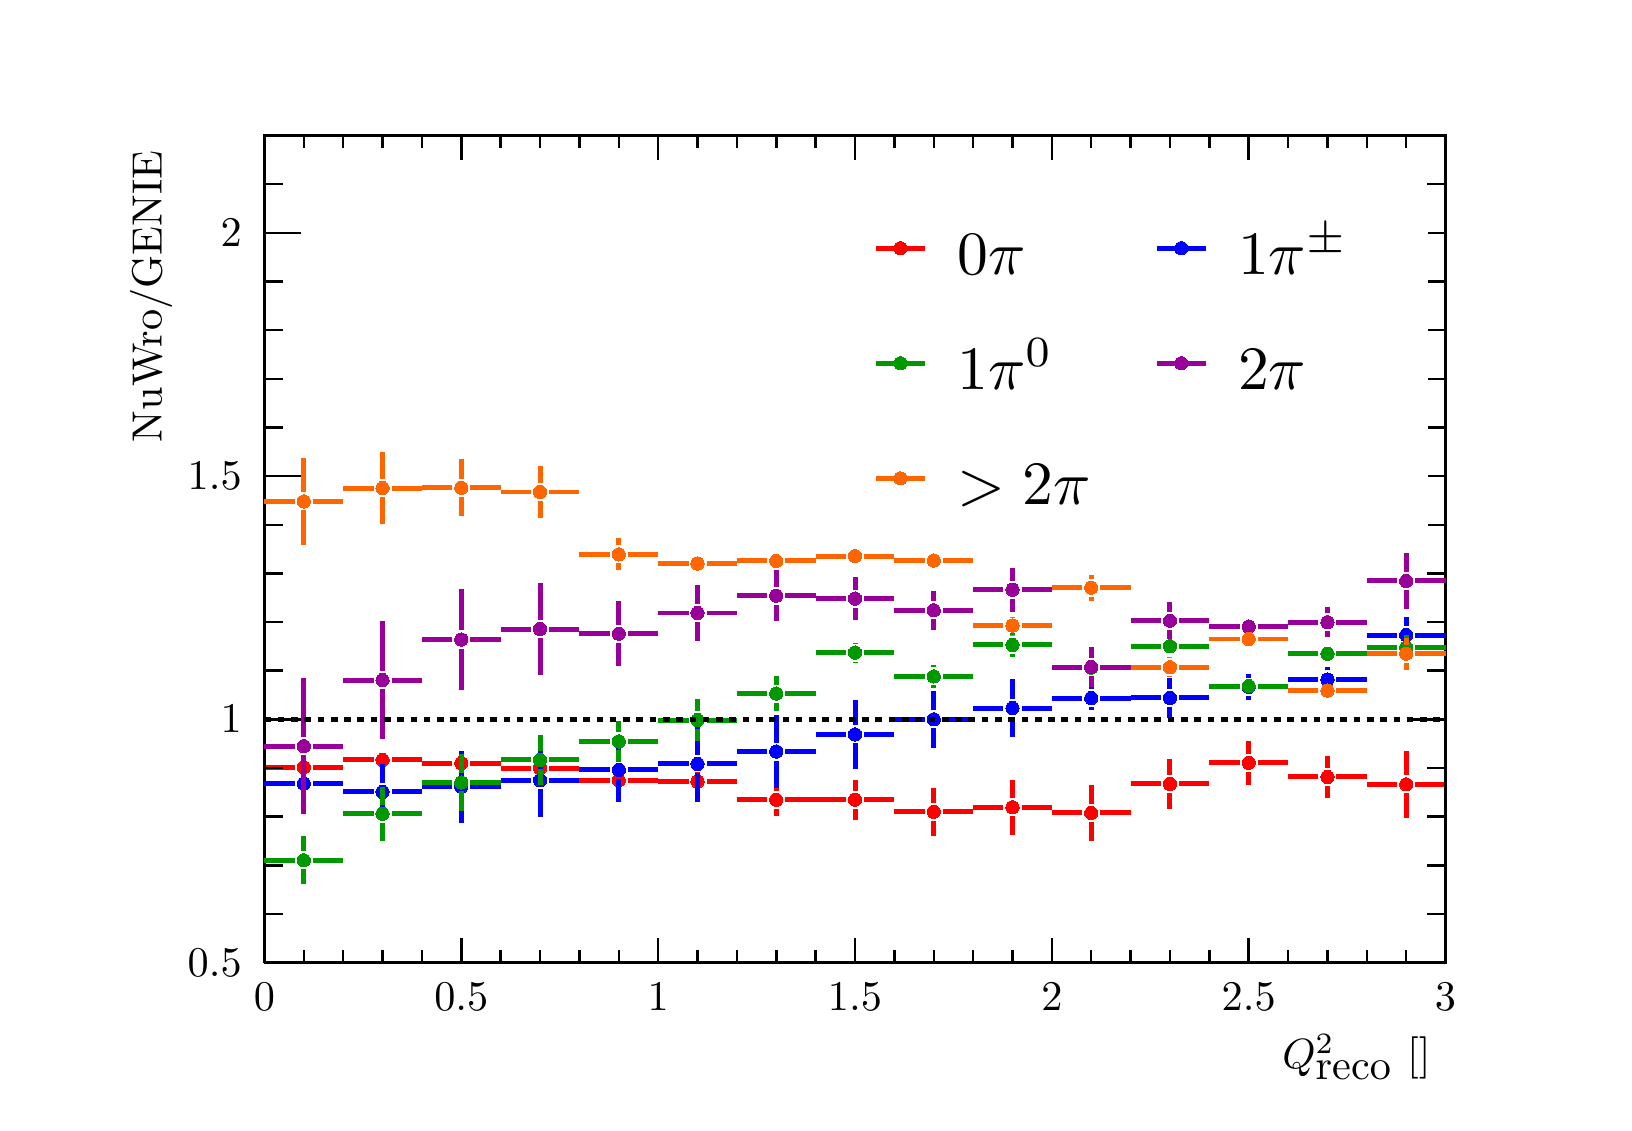
\begin{tikzpicture} 
\pgfdeclareplotmark{cross} {
\pgfpathmoveto{\pgfpoint{-0.3\pgfplotmarksize}{\pgfplotmarksize}}
\pgfpathlineto{\pgfpoint{+0.3\pgfplotmarksize}{\pgfplotmarksize}}
\pgfpathlineto{\pgfpoint{+0.3\pgfplotmarksize}{0.3\pgfplotmarksize}}
\pgfpathlineto{\pgfpoint{+1\pgfplotmarksize}{0.3\pgfplotmarksize}}
\pgfpathlineto{\pgfpoint{+1\pgfplotmarksize}{-0.3\pgfplotmarksize}}
\pgfpathlineto{\pgfpoint{+0.3\pgfplotmarksize}{-0.3\pgfplotmarksize}}
\pgfpathlineto{\pgfpoint{+0.3\pgfplotmarksize}{-1.\pgfplotmarksize}}
\pgfpathlineto{\pgfpoint{-0.3\pgfplotmarksize}{-1.\pgfplotmarksize}}
\pgfpathlineto{\pgfpoint{-0.3\pgfplotmarksize}{-0.3\pgfplotmarksize}}
\pgfpathlineto{\pgfpoint{-1.\pgfplotmarksize}{-0.3\pgfplotmarksize}}
\pgfpathlineto{\pgfpoint{-1.\pgfplotmarksize}{0.3\pgfplotmarksize}}
\pgfpathlineto{\pgfpoint{-0.3\pgfplotmarksize}{0.3\pgfplotmarksize}}
\pgfpathclose
\pgfusepathqstroke
}
\pgfdeclareplotmark{cross*} {
\pgfpathmoveto{\pgfpoint{-0.3\pgfplotmarksize}{\pgfplotmarksize}}
\pgfpathlineto{\pgfpoint{+0.3\pgfplotmarksize}{\pgfplotmarksize}}
\pgfpathlineto{\pgfpoint{+0.3\pgfplotmarksize}{0.3\pgfplotmarksize}}
\pgfpathlineto{\pgfpoint{+1\pgfplotmarksize}{0.3\pgfplotmarksize}}
\pgfpathlineto{\pgfpoint{+1\pgfplotmarksize}{-0.3\pgfplotmarksize}}
\pgfpathlineto{\pgfpoint{+0.3\pgfplotmarksize}{-0.3\pgfplotmarksize}}
\pgfpathlineto{\pgfpoint{+0.3\pgfplotmarksize}{-1.\pgfplotmarksize}}
\pgfpathlineto{\pgfpoint{-0.3\pgfplotmarksize}{-1.\pgfplotmarksize}}
\pgfpathlineto{\pgfpoint{-0.3\pgfplotmarksize}{-0.3\pgfplotmarksize}}
\pgfpathlineto{\pgfpoint{-1.\pgfplotmarksize}{-0.3\pgfplotmarksize}}
\pgfpathlineto{\pgfpoint{-1.\pgfplotmarksize}{0.3\pgfplotmarksize}}
\pgfpathlineto{\pgfpoint{-0.3\pgfplotmarksize}{0.3\pgfplotmarksize}}
\pgfpathclose
\pgfusepathqfillstroke
}
\pgfdeclareplotmark{newstar} {
\pgfpathmoveto{\pgfqpoint{0pt}{\pgfplotmarksize}}
\pgfpathlineto{\pgfqpointpolar{44}{0.5\pgfplotmarksize}}
\pgfpathlineto{\pgfqpointpolar{18}{\pgfplotmarksize}}
\pgfpathlineto{\pgfqpointpolar{-20}{0.5\pgfplotmarksize}}
\pgfpathlineto{\pgfqpointpolar{-54}{\pgfplotmarksize}}
\pgfpathlineto{\pgfqpointpolar{-90}{0.5\pgfplotmarksize}}
\pgfpathlineto{\pgfqpointpolar{234}{\pgfplotmarksize}}
\pgfpathlineto{\pgfqpointpolar{198}{0.5\pgfplotmarksize}}
\pgfpathlineto{\pgfqpointpolar{162}{\pgfplotmarksize}}
\pgfpathlineto{\pgfqpointpolar{134}{0.5\pgfplotmarksize}}
\pgfpathclose
\pgfusepathqstroke
}
\pgfdeclareplotmark{newstar*} {
\pgfpathmoveto{\pgfqpoint{0pt}{\pgfplotmarksize}}
\pgfpathlineto{\pgfqpointpolar{44}{0.5\pgfplotmarksize}}
\pgfpathlineto{\pgfqpointpolar{18}{\pgfplotmarksize}}
\pgfpathlineto{\pgfqpointpolar{-20}{0.5\pgfplotmarksize}}
\pgfpathlineto{\pgfqpointpolar{-54}{\pgfplotmarksize}}
\pgfpathlineto{\pgfqpointpolar{-90}{0.5\pgfplotmarksize}}
\pgfpathlineto{\pgfqpointpolar{234}{\pgfplotmarksize}}
\pgfpathlineto{\pgfqpointpolar{198}{0.5\pgfplotmarksize}}
\pgfpathlineto{\pgfqpointpolar{162}{\pgfplotmarksize}}
\pgfpathlineto{\pgfqpointpolar{134}{0.5\pgfplotmarksize}}
\pgfpathclose
\pgfusepathqfillstroke
}
\definecolor{c}{rgb}{1,1,1};
\draw [color=c, fill=c] (0,0) rectangle (20,13.639);
\draw [color=c, fill=c] (3,1.77307) rectangle (18,12.2751);
\definecolor{c}{rgb}{0,0,0};
\draw [c,line width=0.9] (3,1.77307) -- (3,12.2751) -- (18,12.2751) -- (18,1.77307) -- (3,1.77307);
\definecolor{c}{rgb}{1,1,1};
\draw [color=c, fill=c] (3,1.77307) rectangle (18,12.2751);
\definecolor{c}{rgb}{0,0,0};
\draw [c,line width=0.9] (3,1.77307) -- (3,12.2751) -- (18,12.2751) -- (18,1.77307) -- (3,1.77307);
\definecolor{c}{rgb}{1,0,0};
\draw [c,line width=1.8] (3,4.25421) -- (3.38539,4.25421);
\draw [c,line width=1.8] (3.61461,4.25421) -- (4,4.25421);
\foreach \P in {(3.5,4.25421)}{\draw[mark options={color=c,fill=c},mark size=2.402402pt, line width=0.000000pt, mark=*] plot coordinates {\P};}
\draw [c,line width=1.8] (4,4.34567) -- (4.38539,4.34567);
\draw [c,line width=1.8] (4.61461,4.34567) -- (5,4.34567);
\foreach \P in {(4.5,4.34567)}{\draw[mark options={color=c,fill=c},mark size=2.402402pt, line width=0.000000pt, mark=*] plot coordinates {\P};}
\draw [c,line width=1.8] (5,4.30631) -- (5.38539,4.30631);
\draw [c,line width=1.8] (5.61461,4.30631) -- (6,4.30631);
\foreach \P in {(5.5,4.30631)}{\draw[mark options={color=c,fill=c},mark size=2.402402pt, line width=0.000000pt, mark=*] plot coordinates {\P};}
\draw [c,line width=1.8] (6,4.24171) -- (6.38539,4.24171);
\draw [c,line width=1.8] (6.61461,4.24171) -- (7,4.24171);
\foreach \P in {(6.5,4.24171)}{\draw[mark options={color=c,fill=c},mark size=2.402402pt, line width=0.000000pt, mark=*] plot coordinates {\P};}
\draw [c,line width=1.8] (7,4.08889) -- (7.38539,4.08889);
\draw [c,line width=1.8] (7.61461,4.08889) -- (8,4.08889);
\foreach \P in {(7.5,4.08889)}{\draw[mark options={color=c,fill=c},mark size=2.402402pt, line width=0.000000pt, mark=*] plot coordinates {\P};}
\draw [c,line width=1.8] (8.5,3.95128) -- (8.5,3.95761);
\draw [c,line width=1.8] (8.5,4.18684) -- (8.5,4.19317);
\draw [c,line width=1.8] (8,4.07222) -- (8.38539,4.07222);
\draw [c,line width=1.8] (8.61461,4.07222) -- (9,4.07222);
\foreach \P in {(8.5,4.07222)}{\draw[mark options={color=c,fill=c},mark size=2.402402pt, line width=0.000000pt, mark=*] plot coordinates {\P};}
\draw [c,line width=1.8] (9.5,3.63206) -- (9.5,3.72656);
\draw [c,line width=1.8] (9.5,3.95578) -- (9.5,4.05028);
\draw [c,line width=1.8] (9,3.84117) -- (9.38539,3.84117);
\draw [c,line width=1.8] (9.61461,3.84117) -- (10,3.84117);
\foreach \P in {(9.5,3.84117)}{\draw[mark options={color=c,fill=c},mark size=2.402402pt, line width=0.000000pt, mark=*] plot coordinates {\P};}
\draw [c,line width=1.8] (10.5,3.58793) -- (10.5,3.72697);
\draw [c,line width=1.8] (10.5,3.9562) -- (10.5,4.09523);
\draw [c,line width=1.8] (10,3.84158) -- (10.3854,3.84158);
\draw [c,line width=1.8] (10.6146,3.84158) -- (11,3.84158);
\foreach \P in {(10.5,3.84158)}{\draw[mark options={color=c,fill=c},mark size=2.402402pt, line width=0.000000pt, mark=*] plot coordinates {\P};}
\draw [c,line width=1.8] (11.5,3.38105) -- (11.5,3.57398);
\draw [c,line width=1.8] (11.5,3.8032) -- (11.5,3.99612);
\draw [c,line width=1.8] (11,3.68859) -- (11.3854,3.68859);
\draw [c,line width=1.8] (11.6146,3.68859) -- (12,3.68859);
\foreach \P in {(11.5,3.68859)}{\draw[mark options={color=c,fill=c},mark size=2.402402pt, line width=0.000000pt, mark=*] plot coordinates {\P};}
\draw [c,line width=1.8] (12.5,3.39304) -- (12.5,3.62991);
\draw [c,line width=1.8] (12.5,3.85914) -- (12.5,4.09601);
\draw [c,line width=1.8] (12,3.74452) -- (12.3854,3.74452);
\draw [c,line width=1.8] (12.6146,3.74452) -- (13,3.74452);
\foreach \P in {(12.5,3.74452)}{\draw[mark options={color=c,fill=c},mark size=2.402402pt, line width=0.000000pt, mark=*] plot coordinates {\P};}
\draw [c,line width=1.8] (13.5,3.31572) -- (13.5,3.55841);
\draw [c,line width=1.8] (13.5,3.78764) -- (13.5,4.03034);
\draw [c,line width=1.8] (13,3.67303) -- (13.3854,3.67303);
\draw [c,line width=1.8] (13.6146,3.67303) -- (14,3.67303);
\foreach \P in {(13.5,3.67303)}{\draw[mark options={color=c,fill=c},mark size=2.402402pt, line width=0.000000pt, mark=*] plot coordinates {\P};}
\draw [c,line width=1.8] (14.5,3.72735) -- (14.5,3.92631);
\draw [c,line width=1.8] (14.5,4.15553) -- (14.5,4.35448);
\draw [c,line width=1.8] (14,4.04092) -- (14.3854,4.04092);
\draw [c,line width=1.8] (14.6146,4.04092) -- (15,4.04092);
\foreach \P in {(14.5,4.04092)}{\draw[mark options={color=c,fill=c},mark size=2.402402pt, line width=0.000000pt, mark=*] plot coordinates {\P};}
\draw [c,line width=1.8] (15.5,4.02951) -- (15.5,4.19558);
\draw [c,line width=1.8] (15.5,4.42481) -- (15.5,4.59088);
\draw [c,line width=1.8] (15,4.3102) -- (15.3854,4.3102);
\draw [c,line width=1.8] (15.6146,4.3102) -- (16,4.3102);
\foreach \P in {(15.5,4.3102)}{\draw[mark options={color=c,fill=c},mark size=2.402402pt, line width=0.000000pt, mark=*] plot coordinates {\P};}
\draw [c,line width=1.8] (16.5,3.85896) -- (16.5,4.01508);
\draw [c,line width=1.8] (16.5,4.24431) -- (16.5,4.40042);
\draw [c,line width=1.8] (16,4.12969) -- (16.3854,4.12969);
\draw [c,line width=1.8] (16.6146,4.12969) -- (17,4.12969);
\foreach \P in {(16.5,4.12969)}{\draw[mark options={color=c,fill=c},mark size=2.402402pt, line width=0.000000pt, mark=*] plot coordinates {\P};}
\draw [c,line width=1.8] (17.5,3.61236) -- (17.5,3.92183);
\draw [c,line width=1.8] (17.5,4.15105) -- (17.5,4.46052);
\draw [c,line width=1.8] (17,4.03644) -- (17.3854,4.03644);
\draw [c,line width=1.8] (17.6146,4.03644) -- (18,4.03644);
\foreach \P in {(17.5,4.03644)}{\draw[mark options={color=c,fill=c},mark size=2.402402pt, line width=0.000000pt, mark=*] plot coordinates {\P};}
\definecolor{c}{rgb}{0,0,0};
\draw [c,line width=0.9] (3,1.77307) -- (18,1.77307);
\draw [c,line width=0.9] (3,2.07994) -- (3,1.77307);
\draw [c,line width=0.9] (3.5,1.9265) -- (3.5,1.77307);
\draw [c,line width=0.9] (4,1.9265) -- (4,1.77307);
\draw [c,line width=0.9] (4.5,1.9265) -- (4.5,1.77307);
\draw [c,line width=0.9] (5,1.9265) -- (5,1.77307);
\draw [c,line width=0.9] (5.5,2.07994) -- (5.5,1.77307);
\draw [c,line width=0.9] (6,1.9265) -- (6,1.77307);
\draw [c,line width=0.9] (6.5,1.9265) -- (6.5,1.77307);
\draw [c,line width=0.9] (7,1.9265) -- (7,1.77307);
\draw [c,line width=0.9] (7.5,1.9265) -- (7.5,1.77307);
\draw [c,line width=0.9] (8,2.07994) -- (8,1.77307);
\draw [c,line width=0.9] (8.5,1.9265) -- (8.5,1.77307);
\draw [c,line width=0.9] (9,1.9265) -- (9,1.77307);
\draw [c,line width=0.9] (9.5,1.9265) -- (9.5,1.77307);
\draw [c,line width=0.9] (10,1.9265) -- (10,1.77307);
\draw [c,line width=0.9] (10.5,2.07994) -- (10.5,1.77307);
\draw [c,line width=0.9] (11,1.9265) -- (11,1.77307);
\draw [c,line width=0.9] (11.5,1.9265) -- (11.5,1.77307);
\draw [c,line width=0.9] (12,1.9265) -- (12,1.77307);
\draw [c,line width=0.9] (12.5,1.9265) -- (12.5,1.77307);
\draw [c,line width=0.9] (13,2.07994) -- (13,1.77307);
\draw [c,line width=0.9] (13.5,1.9265) -- (13.5,1.77307);
\draw [c,line width=0.9] (14,1.9265) -- (14,1.77307);
\draw [c,line width=0.9] (14.5,1.9265) -- (14.5,1.77307);
\draw [c,line width=0.9] (15,1.9265) -- (15,1.77307);
\draw [c,line width=0.9] (15.5,2.07994) -- (15.5,1.77307);
\draw [c,line width=0.9] (16,1.9265) -- (16,1.77307);
\draw [c,line width=0.9] (16.5,1.9265) -- (16.5,1.77307);
\draw [c,line width=0.9] (17,1.9265) -- (17,1.77307);
\draw [c,line width=0.9] (17.5,1.9265) -- (17.5,1.77307);
\draw [c,line width=0.9] (18,2.07994) -- (18,1.77307);
\draw [c,line width=0.9] (18,2.07994) -- (18,1.77307);
\draw [anchor=base] (3,1.15931) node[scale=1.52731, color=c, rotate=0]{0};
\draw [anchor=base] (5.5,1.15931) node[scale=1.52731, color=c, rotate=0]{0.5};
\draw [anchor=base] (8,1.15931) node[scale=1.52731, color=c, rotate=0]{1};
\draw [anchor=base] (10.5,1.15931) node[scale=1.52731, color=c, rotate=0]{1.5};
\draw [anchor=base] (13,1.15931) node[scale=1.52731, color=c, rotate=0]{2};
\draw [anchor=base] (15.5,1.15931) node[scale=1.52731, color=c, rotate=0]{2.5};
\draw [anchor=base] (18,1.15931) node[scale=1.52731, color=c, rotate=0]{3};
\draw [anchor= east] (18,0.572837) node[scale=1.52731, color=c, rotate=0]{$Q^{2}_{\textrm{reco}}$ [\si{\GeV\squared}] };
\draw [c,line width=0.9] (3,12.2751) -- (18,12.2751);
\draw [c,line width=0.9] (3,11.9682) -- (3,12.2751);
\draw [c,line width=0.9] (3.5,12.1216) -- (3.5,12.2751);
\draw [c,line width=0.9] (4,12.1216) -- (4,12.2751);
\draw [c,line width=0.9] (4.5,12.1216) -- (4.5,12.2751);
\draw [c,line width=0.9] (5,12.1216) -- (5,12.2751);
\draw [c,line width=0.9] (5.5,11.9682) -- (5.5,12.2751);
\draw [c,line width=0.9] (6,12.1216) -- (6,12.2751);
\draw [c,line width=0.9] (6.5,12.1216) -- (6.5,12.2751);
\draw [c,line width=0.9] (7,12.1216) -- (7,12.2751);
\draw [c,line width=0.9] (7.5,12.1216) -- (7.5,12.2751);
\draw [c,line width=0.9] (8,11.9682) -- (8,12.2751);
\draw [c,line width=0.9] (8.5,12.1216) -- (8.5,12.2751);
\draw [c,line width=0.9] (9,12.1216) -- (9,12.2751);
\draw [c,line width=0.9] (9.5,12.1216) -- (9.5,12.2751);
\draw [c,line width=0.9] (10,12.1216) -- (10,12.2751);
\draw [c,line width=0.9] (10.5,11.9682) -- (10.5,12.2751);
\draw [c,line width=0.9] (11,12.1216) -- (11,12.2751);
\draw [c,line width=0.9] (11.5,12.1216) -- (11.5,12.2751);
\draw [c,line width=0.9] (12,12.1216) -- (12,12.2751);
\draw [c,line width=0.9] (12.5,12.1216) -- (12.5,12.2751);
\draw [c,line width=0.9] (13,11.9682) -- (13,12.2751);
\draw [c,line width=0.9] (13.5,12.1216) -- (13.5,12.2751);
\draw [c,line width=0.9] (14,12.1216) -- (14,12.2751);
\draw [c,line width=0.9] (14.5,12.1216) -- (14.5,12.2751);
\draw [c,line width=0.9] (15,12.1216) -- (15,12.2751);
\draw [c,line width=0.9] (15.5,11.9682) -- (15.5,12.2751);
\draw [c,line width=0.9] (16,12.1216) -- (16,12.2751);
\draw [c,line width=0.9] (16.5,12.1216) -- (16.5,12.2751);
\draw [c,line width=0.9] (17,12.1216) -- (17,12.2751);
\draw [c,line width=0.9] (17.5,12.1216) -- (17.5,12.2751);
\draw [c,line width=0.9] (18,11.9682) -- (18,12.2751);
\draw [c,line width=0.9] (18,11.9682) -- (18,12.2751);
\draw [c,line width=0.9] (3,1.77307) -- (3,12.2751);
\draw [c,line width=0.9] (3.462,1.77307) -- (3,1.77307);
\draw [c,line width=0.9] (3.231,2.39083) -- (3,2.39083);
\draw [c,line width=0.9] (3.231,3.0086) -- (3,3.0086);
\draw [c,line width=0.9] (3.231,3.62636) -- (3,3.62636);
\draw [c,line width=0.9] (3.231,4.24413) -- (3,4.24413);
\draw [c,line width=0.9] (3.462,4.86189) -- (3,4.86189);
\draw [c,line width=0.9] (3.231,5.47966) -- (3,5.47966);
\draw [c,line width=0.9] (3.231,6.09742) -- (3,6.09742);
\draw [c,line width=0.9] (3.231,6.71519) -- (3,6.71519);
\draw [c,line width=0.9] (3.231,7.33295) -- (3,7.33295);
\draw [c,line width=0.9] (3.462,7.95072) -- (3,7.95072);
\draw [c,line width=0.9] (3.231,8.56848) -- (3,8.56848);
\draw [c,line width=0.9] (3.231,9.18625) -- (3,9.18625);
\draw [c,line width=0.9] (3.231,9.80401) -- (3,9.80401);
\draw [c,line width=0.9] (3.231,10.4218) -- (3,10.4218);
\draw [c,line width=0.9] (3.462,11.0395) -- (3,11.0395);
\draw [c,line width=0.9] (3.462,11.0395) -- (3,11.0395);
\draw [c,line width=0.9] (3.231,11.6573) -- (3,11.6573);
\draw [c,line width=0.9] (3.231,12.2751) -- (3,12.2751);
\draw [anchor= east] (2.9,1.77307) node[scale=1.52731, color=c, rotate=0]{0.5};
\draw [anchor= east] (2.9,4.86189) node[scale=1.52731, color=c, rotate=0]{1};
\draw [anchor= east] (2.9,7.95072) node[scale=1.52731, color=c, rotate=0]{1.5};
\draw [anchor= east] (2.9,11.0395) node[scale=1.52731, color=c, rotate=0]{2};
\draw [anchor= east] (1.56,12.2751) node[scale=1.52731, color=c, rotate=90]{ NuWro/GENIE};
\draw [c,line width=0.9] (18,1.77307) -- (18,12.2751);
\draw [c,line width=0.9] (17.538,1.77307) -- (18,1.77307);
\draw [c,line width=0.9] (17.769,2.39083) -- (18,2.39083);
\draw [c,line width=0.9] (17.769,3.0086) -- (18,3.0086);
\draw [c,line width=0.9] (17.769,3.62636) -- (18,3.62636);
\draw [c,line width=0.9] (17.769,4.24413) -- (18,4.24413);
\draw [c,line width=0.9] (17.538,4.86189) -- (18,4.86189);
\draw [c,line width=0.9] (17.769,5.47966) -- (18,5.47966);
\draw [c,line width=0.9] (17.769,6.09742) -- (18,6.09742);
\draw [c,line width=0.9] (17.769,6.71519) -- (18,6.71519);
\draw [c,line width=0.9] (17.769,7.33295) -- (18,7.33295);
\draw [c,line width=0.9] (17.538,7.95072) -- (18,7.95072);
\draw [c,line width=0.9] (17.769,8.56848) -- (18,8.56848);
\draw [c,line width=0.9] (17.769,9.18625) -- (18,9.18625);
\draw [c,line width=0.9] (17.769,9.80401) -- (18,9.80401);
\draw [c,line width=0.9] (17.769,10.4218) -- (18,10.4218);
\draw [c,line width=0.9] (17.538,11.0395) -- (18,11.0395);
\draw [c,line width=0.9] (17.538,11.0395) -- (18,11.0395);
\draw [c,line width=0.9] (17.769,11.6573) -- (18,11.6573);
\draw [c,line width=0.9] (17.769,12.2751) -- (18,12.2751);
\definecolor{c}{rgb}{0,0,1};
\draw [c,line width=1.8] (3.5,3.85564) -- (3.5,3.93025);
\draw [c,line width=1.8] (3.5,4.15947) -- (3.5,4.23409);
\draw [c,line width=1.8] (3,4.04486) -- (3.38539,4.04486);
\draw [c,line width=1.8] (3.61461,4.04486) -- (4,4.04486);
\foreach \P in {(3.5,4.04486)}{\draw[mark options={color=c,fill=c},mark size=2.402402pt, line width=0.000000pt, mark=*] plot coordinates {\P};}
\draw [c,line width=1.8] (4.5,3.58177) -- (4.5,3.82528);
\draw [c,line width=1.8] (4.5,4.05451) -- (4.5,4.29802);
\draw [c,line width=1.8] (4,3.93989) -- (4.38539,3.93989);
\draw [c,line width=1.8] (4.61461,3.93989) -- (5,3.93989);
\foreach \P in {(4.5,3.93989)}{\draw[mark options={color=c,fill=c},mark size=2.402402pt, line width=0.000000pt, mark=*] plot coordinates {\P};}
\draw [c,line width=1.8] (5.5,3.55128) -- (5.5,3.892);
\draw [c,line width=1.8] (5.5,4.12123) -- (5.5,4.46194);
\draw [c,line width=1.8] (5,4.00661) -- (5.38539,4.00661);
\draw [c,line width=1.8] (5.61461,4.00661) -- (6,4.00661);
\foreach \P in {(5.5,4.00661)}{\draw[mark options={color=c,fill=c},mark size=2.402402pt, line width=0.000000pt, mark=*] plot coordinates {\P};}
\draw [c,line width=1.8] (6.5,3.62757) -- (6.5,3.97413);
\draw [c,line width=1.8] (6.5,4.20336) -- (6.5,4.54993);
\draw [c,line width=1.8] (6,4.08875) -- (6.38539,4.08875);
\draw [c,line width=1.8] (6.61461,4.08875) -- (7,4.08875);
\foreach \P in {(6.5,4.08875)}{\draw[mark options={color=c,fill=c},mark size=2.402402pt, line width=0.000000pt, mark=*] plot coordinates {\P};}
\draw [c,line width=1.8] (7.5,3.81352) -- (7.5,4.10518);
\draw [c,line width=1.8] (7.5,4.3344) -- (7.5,4.62606);
\draw [c,line width=1.8] (7,4.21979) -- (7.38539,4.21979);
\draw [c,line width=1.8] (7.61461,4.21979) -- (8,4.21979);
\foreach \P in {(7.5,4.21979)}{\draw[mark options={color=c,fill=c},mark size=2.402402pt, line width=0.000000pt, mark=*] plot coordinates {\P};}
\draw [c,line width=1.8] (8.5,3.81693) -- (8.5,4.18106);
\draw [c,line width=1.8] (8.5,4.41029) -- (8.5,4.77442);
\draw [c,line width=1.8] (8,4.29568) -- (8.38539,4.29568);
\draw [c,line width=1.8] (8.61461,4.29568) -- (9,4.29568);
\foreach \P in {(8.5,4.29568)}{\draw[mark options={color=c,fill=c},mark size=2.402402pt, line width=0.000000pt, mark=*] plot coordinates {\P};}
\draw [c,line width=1.8] (9.5,3.98934) -- (9.5,4.33832);
\draw [c,line width=1.8] (9.5,4.56755) -- (9.5,4.91652);
\draw [c,line width=1.8] (9,4.45293) -- (9.38539,4.45293);
\draw [c,line width=1.8] (9.61461,4.45293) -- (10,4.45293);
\foreach \P in {(9.5,4.45293)}{\draw[mark options={color=c,fill=c},mark size=2.402402pt, line width=0.000000pt, mark=*] plot coordinates {\P};}
\draw [c,line width=1.8] (10.5,4.23524) -- (10.5,4.55537);
\draw [c,line width=1.8] (10.5,4.7846) -- (10.5,5.10473);
\draw [c,line width=1.8] (10,4.66999) -- (10.3854,4.66999);
\draw [c,line width=1.8] (10.6146,4.66999) -- (11,4.66999);
\foreach \P in {(10.5,4.66999)}{\draw[mark options={color=c,fill=c},mark size=2.402402pt, line width=0.000000pt, mark=*] plot coordinates {\P};}
\draw [c,line width=1.8] (11.5,4.49798) -- (11.5,4.74711);
\draw [c,line width=1.8] (11.5,4.97634) -- (11.5,5.22547);
\draw [c,line width=1.8] (11,4.86172) -- (11.3854,4.86172);
\draw [c,line width=1.8] (11.6146,4.86172) -- (12,4.86172);
\foreach \P in {(11.5,4.86172)}{\draw[mark options={color=c,fill=c},mark size=2.402402pt, line width=0.000000pt, mark=*] plot coordinates {\P};}
\draw [c,line width=1.8] (12.5,4.63848) -- (12.5,4.89032);
\draw [c,line width=1.8] (12.5,5.11954) -- (12.5,5.37138);
\draw [c,line width=1.8] (12,5.00493) -- (12.3854,5.00493);
\draw [c,line width=1.8] (12.6146,5.00493) -- (13,5.00493);
\foreach \P in {(12.5,5.00493)}{\draw[mark options={color=c,fill=c},mark size=2.402402pt, line width=0.000000pt, mark=*] plot coordinates {\P};}
\draw [c,line width=1.8] (13.5,4.97669) -- (13.5,5.01721);
\draw [c,line width=1.8] (13.5,5.24644) -- (13.5,5.28695);
\draw [c,line width=1.8] (13,5.13182) -- (13.3854,5.13182);
\draw [c,line width=1.8] (13.6146,5.13182) -- (14,5.13182);
\foreach \P in {(13.5,5.13182)}{\draw[mark options={color=c,fill=c},mark size=2.402402pt, line width=0.000000pt, mark=*] plot coordinates {\P};}
\draw [c,line width=1.8] (14.5,4.88157) -- (14.5,5.01984);
\draw [c,line width=1.8] (14.5,5.24906) -- (14.5,5.38732);
\draw [c,line width=1.8] (14,5.13445) -- (14.3854,5.13445);
\draw [c,line width=1.8] (14.6146,5.13445) -- (15,5.13445);
\foreach \P in {(14.5,5.13445)}{\draw[mark options={color=c,fill=c},mark size=2.402402pt, line width=0.000000pt, mark=*] plot coordinates {\P};}
\draw [c,line width=1.8] (15.5,5.10808) -- (15.5,5.1601);
\draw [c,line width=1.8] (15.5,5.38933) -- (15.5,5.44135);
\draw [c,line width=1.8] (15,5.27471) -- (15.3854,5.27471);
\draw [c,line width=1.8] (15.6146,5.27471) -- (16,5.27471);
\foreach \P in {(15.5,5.27471)}{\draw[mark options={color=c,fill=c},mark size=2.402402pt, line width=0.000000pt, mark=*] plot coordinates {\P};}
\draw [c,line width=1.8] (16.5,5.2049) -- (16.5,5.25334);
\draw [c,line width=1.8] (16.5,5.48257) -- (16.5,5.531);
\draw [c,line width=1.8] (16,5.36795) -- (16.3854,5.36795);
\draw [c,line width=1.8] (16.6146,5.36795) -- (17,5.36795);
\foreach \P in {(16.5,5.36795)}{\draw[mark options={color=c,fill=c},mark size=2.402402pt, line width=0.000000pt, mark=*] plot coordinates {\P};}
\draw [c,line width=1.8] (17.5,5.70018) -- (17.5,5.81797);
\draw [c,line width=1.8] (17.5,6.0472) -- (17.5,6.16499);
\draw [c,line width=1.8] (17,5.93258) -- (17.3854,5.93258);
\draw [c,line width=1.8] (17.6146,5.93258) -- (18,5.93258);
\foreach \P in {(17.5,5.93258)}{\draw[mark options={color=c,fill=c},mark size=2.402402pt, line width=0.000000pt, mark=*] plot coordinates {\P};}
\definecolor{c}{rgb}{0,0.6,0};
\draw [c,line width=1.8] (3.5,2.76788) -- (3.5,2.95756);
\draw [c,line width=1.8] (3.5,3.18679) -- (3.5,3.37647);
\draw [c,line width=1.8] (3,3.07217) -- (3.38539,3.07217);
\draw [c,line width=1.8] (3.61461,3.07217) -- (4,3.07217);
\foreach \P in {(3.5,3.07217)}{\draw[mark options={color=c,fill=c},mark size=2.402402pt, line width=0.000000pt, mark=*] plot coordinates {\P};}
\draw [c,line width=1.8] (4.5,3.32244) -- (4.5,3.54829);
\draw [c,line width=1.8] (4.5,3.77752) -- (4.5,4.00337);
\draw [c,line width=1.8] (4,3.6629) -- (4.38539,3.6629);
\draw [c,line width=1.8] (4.61461,3.6629) -- (5,3.6629);
\foreach \P in {(4.5,3.6629)}{\draw[mark options={color=c,fill=c},mark size=2.402402pt, line width=0.000000pt, mark=*] plot coordinates {\P};}
\draw [c,line width=1.8] (5.5,3.70004) -- (5.5,3.94594);
\draw [c,line width=1.8] (5.5,4.17516) -- (5.5,4.42106);
\draw [c,line width=1.8] (5,4.06055) -- (5.38539,4.06055);
\draw [c,line width=1.8] (5.61461,4.06055) -- (6,4.06055);
\foreach \P in {(5.5,4.06055)}{\draw[mark options={color=c,fill=c},mark size=2.402402pt, line width=0.000000pt, mark=*] plot coordinates {\P};}
\draw [c,line width=1.8] (6.5,4.02444) -- (6.5,4.23098);
\draw [c,line width=1.8] (6.5,4.46021) -- (6.5,4.66675);
\draw [c,line width=1.8] (6,4.3456) -- (6.38539,4.3456);
\draw [c,line width=1.8] (6.61461,4.3456) -- (7,4.3456);
\foreach \P in {(6.5,4.3456)}{\draw[mark options={color=c,fill=c},mark size=2.402402pt, line width=0.000000pt, mark=*] plot coordinates {\P};}
\draw [c,line width=1.8] (7.5,4.3251) -- (7.5,4.46706);
\draw [c,line width=1.8] (7.5,4.69629) -- (7.5,4.83825);
\draw [c,line width=1.8] (7,4.58167) -- (7.38539,4.58167);
\draw [c,line width=1.8] (7.61461,4.58167) -- (8,4.58167);
\foreach \P in {(7.5,4.58167)}{\draw[mark options={color=c,fill=c},mark size=2.402402pt, line width=0.000000pt, mark=*] plot coordinates {\P};}
\draw [c,line width=1.8] (8.5,4.58307) -- (8.5,4.73735);
\draw [c,line width=1.8] (8.5,4.96658) -- (8.5,5.12086);
\draw [c,line width=1.8] (8,4.85196) -- (8.38539,4.85196);
\draw [c,line width=1.8] (8.61461,4.85196) -- (9,4.85196);
\foreach \P in {(8.5,4.85196)}{\draw[mark options={color=c,fill=c},mark size=2.402402pt, line width=0.000000pt, mark=*] plot coordinates {\P};}
\draw [c,line width=1.8] (9.5,4.96684) -- (9.5,5.07409);
\draw [c,line width=1.8] (9.5,5.30332) -- (9.5,5.41058);
\draw [c,line width=1.8] (9,5.18871) -- (9.38539,5.18871);
\draw [c,line width=1.8] (9.61461,5.18871) -- (10,5.18871);
\foreach \P in {(9.5,5.18871)}{\draw[mark options={color=c,fill=c},mark size=2.402402pt, line width=0.000000pt, mark=*] plot coordinates {\P};}
\draw [c,line width=1.8] (10.5,5.58259) -- (10.5,5.59515);
\draw [c,line width=1.8] (10.5,5.82437) -- (10.5,5.83693);
\draw [c,line width=1.8] (10,5.70976) -- (10.3854,5.70976);
\draw [c,line width=1.8] (10.6146,5.70976) -- (11,5.70976);
\foreach \P in {(10.5,5.70976)}{\draw[mark options={color=c,fill=c},mark size=2.402402pt, line width=0.000000pt, mark=*] plot coordinates {\P};}
\draw [c,line width=1.8] (11.5,5.26367) -- (11.5,5.29283);
\draw [c,line width=1.8] (11.5,5.52206) -- (11.5,5.55123);
\draw [c,line width=1.8] (11,5.40745) -- (11.3854,5.40745);
\draw [c,line width=1.8] (11.6146,5.40745) -- (12,5.40745);
\foreach \P in {(11.5,5.40745)}{\draw[mark options={color=c,fill=c},mark size=2.402402pt, line width=0.000000pt, mark=*] plot coordinates {\P};}
\draw [c,line width=1.8] (12.5,5.65917) -- (12.5,5.69177);
\draw [c,line width=1.8] (12.5,5.921) -- (12.5,5.95361);
\draw [c,line width=1.8] (12,5.80639) -- (12.3854,5.80639);
\draw [c,line width=1.8] (12.6146,5.80639) -- (13,5.80639);
\foreach \P in {(12.5,5.80639)}{\draw[mark options={color=c,fill=c},mark size=2.402402pt, line width=0.000000pt, mark=*] plot coordinates {\P};}
\draw [c,line width=1.8] (13,5.51858) -- (13.3854,5.51858);
\draw [c,line width=1.8] (13.6146,5.51858) -- (14,5.51858);
\foreach \P in {(13.5,5.51858)}{\draw[mark options={color=c,fill=c},mark size=2.402402pt, line width=0.000000pt, mark=*] plot coordinates {\P};}
\draw [c,line width=1.8] (14,5.79098) -- (14.3854,5.79098);
\draw [c,line width=1.8] (14.6146,5.79098) -- (15,5.79098);
\foreach \P in {(14.5,5.79098)}{\draw[mark options={color=c,fill=c},mark size=2.402402pt, line width=0.000000pt, mark=*] plot coordinates {\P};}
\draw [c,line width=1.8] (15,5.28459) -- (15.3854,5.28459);
\draw [c,line width=1.8] (15.6146,5.28459) -- (16,5.28459);
\foreach \P in {(15.5,5.28459)}{\draw[mark options={color=c,fill=c},mark size=2.402402pt, line width=0.000000pt, mark=*] plot coordinates {\P};}
\draw [c,line width=1.8] (16,5.6943) -- (16.3854,5.6943);
\draw [c,line width=1.8] (16.6146,5.6943) -- (17,5.6943);
\foreach \P in {(16.5,5.6943)}{\draw[mark options={color=c,fill=c},mark size=2.402402pt, line width=0.000000pt, mark=*] plot coordinates {\P};}
\draw [c,line width=1.8] (17.5,5.61317) -- (17.5,5.65889);
\draw [c,line width=1.8] (17.5,5.88811) -- (17.5,5.93383);
\draw [c,line width=1.8] (17,5.7735) -- (17.3854,5.7735);
\draw [c,line width=1.8] (17.6146,5.7735) -- (18,5.7735);
\foreach \P in {(17.5,5.7735)}{\draw[mark options={color=c,fill=c},mark size=2.402402pt, line width=0.000000pt, mark=*] plot coordinates {\P};}
\definecolor{c}{rgb}{0.6,0,0.6};
\draw [c,line width=1.8] (3.5,3.65904) -- (3.5,4.4065);
\draw [c,line width=1.8] (3.5,4.63573) -- (3.5,5.38318);
\draw [c,line width=1.8] (3,4.52111) -- (3.38539,4.52111);
\draw [c,line width=1.8] (3.61461,4.52111) -- (4,4.52111);
\foreach \P in {(3.5,4.52111)}{\draw[mark options={color=c,fill=c},mark size=2.402402pt, line width=0.000000pt, mark=*] plot coordinates {\P};}
\draw [c,line width=1.8] (4.5,4.60862) -- (4.5,5.24532);
\draw [c,line width=1.8] (4.5,5.47454) -- (4.5,6.11124);
\draw [c,line width=1.8] (4,5.35993) -- (4.38539,5.35993);
\draw [c,line width=1.8] (4.61461,5.35993) -- (5,5.35993);
\foreach \P in {(4.5,5.35993)}{\draw[mark options={color=c,fill=c},mark size=2.402402pt, line width=0.000000pt, mark=*] plot coordinates {\P};}
\draw [c,line width=1.8] (5.5,5.2307) -- (5.5,5.76088);
\draw [c,line width=1.8] (5.5,5.9901) -- (5.5,6.52028);
\draw [c,line width=1.8] (5,5.87549) -- (5.38539,5.87549);
\draw [c,line width=1.8] (5.61461,5.87549) -- (6,5.87549);
\foreach \P in {(5.5,5.87549)}{\draw[mark options={color=c,fill=c},mark size=2.402402pt, line width=0.000000pt, mark=*] plot coordinates {\P};}
\draw [c,line width=1.8] (6.5,5.41876) -- (6.5,5.8942);
\draw [c,line width=1.8] (6.5,6.12343) -- (6.5,6.59886);
\draw [c,line width=1.8] (6,6.00881) -- (6.38539,6.00881);
\draw [c,line width=1.8] (6.61461,6.00881) -- (7,6.00881);
\foreach \P in {(6.5,6.00881)}{\draw[mark options={color=c,fill=c},mark size=2.402402pt, line width=0.000000pt, mark=*] plot coordinates {\P};}
\draw [c,line width=1.8] (7.5,5.53892) -- (7.5,5.83474);
\draw [c,line width=1.8] (7.5,6.06397) -- (7.5,6.3598);
\draw [c,line width=1.8] (7,5.94936) -- (7.38539,5.94936);
\draw [c,line width=1.8] (7.61461,5.94936) -- (8,5.94936);
\foreach \P in {(7.5,5.94936)}{\draw[mark options={color=c,fill=c},mark size=2.402402pt, line width=0.000000pt, mark=*] plot coordinates {\P};}
\draw [c,line width=1.8] (8.5,5.86292) -- (8.5,6.0977);
\draw [c,line width=1.8] (8.5,6.32692) -- (8.5,6.5617);
\draw [c,line width=1.8] (8,6.21231) -- (8.38539,6.21231);
\draw [c,line width=1.8] (8.61461,6.21231) -- (9,6.21231);
\foreach \P in {(8.5,6.21231)}{\draw[mark options={color=c,fill=c},mark size=2.402402pt, line width=0.000000pt, mark=*] plot coordinates {\P};}
\draw [c,line width=1.8] (9.5,6.11151) -- (9.5,6.31766);
\draw [c,line width=1.8] (9.5,6.54689) -- (9.5,6.75304);
\draw [c,line width=1.8] (9,6.43227) -- (9.38539,6.43227);
\draw [c,line width=1.8] (9.61461,6.43227) -- (10,6.43227);
\foreach \P in {(9.5,6.43227)}{\draw[mark options={color=c,fill=c},mark size=2.402402pt, line width=0.000000pt, mark=*] plot coordinates {\P};}
\draw [c,line width=1.8] (10.5,6.11706) -- (10.5,6.28095);
\draw [c,line width=1.8] (10.5,6.51018) -- (10.5,6.67407);
\draw [c,line width=1.8] (10,6.39557) -- (10.3854,6.39557);
\draw [c,line width=1.8] (10.6146,6.39557) -- (11,6.39557);
\foreach \P in {(10.5,6.39557)}{\draw[mark options={color=c,fill=c},mark size=2.402402pt, line width=0.000000pt, mark=*] plot coordinates {\P};}
\draw [c,line width=1.8] (11.5,6.00011) -- (11.5,6.13244);
\draw [c,line width=1.8] (11.5,6.36167) -- (11.5,6.49401);
\draw [c,line width=1.8] (11,6.24706) -- (11.3854,6.24706);
\draw [c,line width=1.8] (11.6146,6.24706) -- (12,6.24706);
\foreach \P in {(11.5,6.24706)}{\draw[mark options={color=c,fill=c},mark size=2.402402pt, line width=0.000000pt, mark=*] plot coordinates {\P};}
\draw [c,line width=1.8] (12.5,6.23056) -- (12.5,6.39411);
\draw [c,line width=1.8] (12.5,6.62333) -- (12.5,6.78688);
\draw [c,line width=1.8] (12,6.50872) -- (12.3854,6.50872);
\draw [c,line width=1.8] (12.6146,6.50872) -- (13,6.50872);
\foreach \P in {(12.5,6.50872)}{\draw[mark options={color=c,fill=c},mark size=2.402402pt, line width=0.000000pt, mark=*] plot coordinates {\P};}
\draw [c,line width=1.8] (13.5,5.27082) -- (13.5,5.4117);
\draw [c,line width=1.8] (13.5,5.64093) -- (13.5,5.78181);
\draw [c,line width=1.8] (13,5.52632) -- (13.3854,5.52632);
\draw [c,line width=1.8] (13.6146,5.52632) -- (14,5.52632);
\foreach \P in {(13.5,5.52632)}{\draw[mark options={color=c,fill=c},mark size=2.402402pt, line width=0.000000pt, mark=*] plot coordinates {\P};}
\draw [c,line width=1.8] (14.5,5.88151) -- (14.5,5.99948);
\draw [c,line width=1.8] (14.5,6.2287) -- (14.5,6.34667);
\draw [c,line width=1.8] (14,6.11409) -- (14.3854,6.11409);
\draw [c,line width=1.8] (14.6146,6.11409) -- (15,6.11409);
\foreach \P in {(14.5,6.11409)}{\draw[mark options={color=c,fill=c},mark size=2.402402pt, line width=0.000000pt, mark=*] plot coordinates {\P};}
\draw [c,line width=1.8] (15,6.03899) -- (15.3854,6.03899);
\draw [c,line width=1.8] (15.6146,6.03899) -- (16,6.03899);
\foreach \P in {(15.5,6.03899)}{\draw[mark options={color=c,fill=c},mark size=2.402402pt, line width=0.000000pt, mark=*] plot coordinates {\P};}
\draw [c,line width=1.8] (16.5,5.90295) -- (16.5,5.97987);
\draw [c,line width=1.8] (16.5,6.2091) -- (16.5,6.28602);
\draw [c,line width=1.8] (16,6.09448) -- (16.3854,6.09448);
\draw [c,line width=1.8] (16.6146,6.09448) -- (17,6.09448);
\foreach \P in {(16.5,6.09448)}{\draw[mark options={color=c,fill=c},mark size=2.402402pt, line width=0.000000pt, mark=*] plot coordinates {\P};}
\draw [c,line width=1.8] (17.5,6.26807) -- (17.5,6.50446);
\draw [c,line width=1.8] (17.5,6.73369) -- (17.5,6.97007);
\draw [c,line width=1.8] (17,6.61907) -- (17.3854,6.61907);
\draw [c,line width=1.8] (17.6146,6.61907) -- (18,6.61907);
\foreach \P in {(17.5,6.61907)}{\draw[mark options={color=c,fill=c},mark size=2.402402pt, line width=0.000000pt, mark=*] plot coordinates {\P};}
\definecolor{c}{rgb}{1,0.4,0};
\draw [c,line width=1.8] (3.5,7.0761) -- (3.5,7.51515);
\draw [c,line width=1.8] (3.5,7.74437) -- (3.5,8.18343);
\draw [c,line width=1.8] (3,7.62976) -- (3.38539,7.62976);
\draw [c,line width=1.8] (3.61461,7.62976) -- (4,7.62976);
\foreach \P in {(3.5,7.62976)}{\draw[mark options={color=c,fill=c},mark size=2.402402pt, line width=0.000000pt, mark=*] plot coordinates {\P};}
\draw [c,line width=1.8] (4.5,7.33943) -- (4.5,7.68486);
\draw [c,line width=1.8] (4.5,7.91409) -- (4.5,8.25952);
\draw [c,line width=1.8] (4,7.79948) -- (4.38539,7.79948);
\draw [c,line width=1.8] (4.61461,7.79948) -- (5,7.79948);
\foreach \P in {(4.5,7.79948)}{\draw[mark options={color=c,fill=c},mark size=2.402402pt, line width=0.000000pt, mark=*] plot coordinates {\P};}
\draw [c,line width=1.8] (5.5,7.43854) -- (5.5,7.68771);
\draw [c,line width=1.8] (5.5,7.91694) -- (5.5,8.16611);
\draw [c,line width=1.8] (5,7.80233) -- (5.38539,7.80233);
\draw [c,line width=1.8] (5.61461,7.80233) -- (6,7.80233);
\foreach \P in {(5.5,7.80233)}{\draw[mark options={color=c,fill=c},mark size=2.402402pt, line width=0.000000pt, mark=*] plot coordinates {\P};}
\draw [c,line width=1.8] (6.5,7.42027) -- (6.5,7.63444);
\draw [c,line width=1.8] (6.5,7.86367) -- (6.5,8.07783);
\draw [c,line width=1.8] (6,7.74905) -- (6.38539,7.74905);
\draw [c,line width=1.8] (6.61461,7.74905) -- (7,7.74905);
\foreach \P in {(6.5,7.74905)}{\draw[mark options={color=c,fill=c},mark size=2.402402pt, line width=0.000000pt, mark=*] plot coordinates {\P};}
\draw [c,line width=1.8] (7.5,6.75391) -- (7.5,6.84229);
\draw [c,line width=1.8] (7.5,7.07151) -- (7.5,7.15989);
\draw [c,line width=1.8] (7,6.9569) -- (7.38539,6.9569);
\draw [c,line width=1.8] (7.61461,6.9569) -- (8,6.9569);
\foreach \P in {(7.5,6.9569)}{\draw[mark options={color=c,fill=c},mark size=2.402402pt, line width=0.000000pt, mark=*] plot coordinates {\P};}
\draw [c,line width=1.8] (8,6.84052) -- (8.38539,6.84052);
\draw [c,line width=1.8] (8.61461,6.84052) -- (9,6.84052);
\foreach \P in {(8.5,6.84052)}{\draw[mark options={color=c,fill=c},mark size=2.402402pt, line width=0.000000pt, mark=*] plot coordinates {\P};}
\draw [c,line width=1.8] (9,6.87444) -- (9.38539,6.87444);
\draw [c,line width=1.8] (9.61461,6.87444) -- (10,6.87444);
\foreach \P in {(9.5,6.87444)}{\draw[mark options={color=c,fill=c},mark size=2.402402pt, line width=0.000000pt, mark=*] plot coordinates {\P};}
\draw [c,line width=1.8] (10,6.93446) -- (10.3854,6.93446);
\draw [c,line width=1.8] (10.6146,6.93446) -- (11,6.93446);
\foreach \P in {(10.5,6.93446)}{\draw[mark options={color=c,fill=c},mark size=2.402402pt, line width=0.000000pt, mark=*] plot coordinates {\P};}
\draw [c,line width=1.8] (11,6.87773) -- (11.3854,6.87773);
\draw [c,line width=1.8] (11.6146,6.87773) -- (12,6.87773);
\foreach \P in {(11.5,6.87773)}{\draw[mark options={color=c,fill=c},mark size=2.402402pt, line width=0.000000pt, mark=*] plot coordinates {\P};}
\draw [c,line width=1.8] (12.5,5.93722) -- (12.5,5.93786);
\draw [c,line width=1.8] (12.5,6.16708) -- (12.5,6.16772);
\draw [c,line width=1.8] (12,6.05247) -- (12.3854,6.05247);
\draw [c,line width=1.8] (12.6146,6.05247) -- (13,6.05247);
\foreach \P in {(12.5,6.05247)}{\draw[mark options={color=c,fill=c},mark size=2.402402pt, line width=0.000000pt, mark=*] plot coordinates {\P};}
\draw [c,line width=1.8] (13.5,6.36843) -- (13.5,6.4196);
\draw [c,line width=1.8] (13.5,6.64883) -- (13.5,6.70001);
\draw [c,line width=1.8] (13,6.53422) -- (13.3854,6.53422);
\draw [c,line width=1.8] (13.6146,6.53422) -- (14,6.53422);
\foreach \P in {(13.5,6.53422)}{\draw[mark options={color=c,fill=c},mark size=2.402402pt, line width=0.000000pt, mark=*] plot coordinates {\P};}
\draw [c,line width=1.8] (14.5,5.39621) -- (14.5,5.40926);
\draw [c,line width=1.8] (14.5,5.63848) -- (14.5,5.65153);
\draw [c,line width=1.8] (14,5.52387) -- (14.3854,5.52387);
\draw [c,line width=1.8] (14.6146,5.52387) -- (15,5.52387);
\foreach \P in {(14.5,5.52387)}{\draw[mark options={color=c,fill=c},mark size=2.402402pt, line width=0.000000pt, mark=*] plot coordinates {\P};}
\draw [c,line width=1.8] (15,5.88208) -- (15.3854,5.88208);
\draw [c,line width=1.8] (15.6146,5.88208) -- (16,5.88208);
\foreach \P in {(15.5,5.88208)}{\draw[mark options={color=c,fill=c},mark size=2.402402pt, line width=0.000000pt, mark=*] plot coordinates {\P};}
\draw [c,line width=1.8] (16,5.22624) -- (16.3854,5.22624);
\draw [c,line width=1.8] (16.6146,5.22624) -- (17,5.22624);
\foreach \P in {(16.5,5.22624)}{\draw[mark options={color=c,fill=c},mark size=2.402402pt, line width=0.000000pt, mark=*] plot coordinates {\P};}
\draw [c,line width=1.8] (17.5,5.49105) -- (17.5,5.58116);
\draw [c,line width=1.8] (17.5,5.81039) -- (17.5,5.9005);
\draw [c,line width=1.8] (17,5.69577) -- (17.3854,5.69577);
\draw [c,line width=1.8] (17.6146,5.69577) -- (18,5.69577);
\foreach \P in {(17.5,5.69577)}{\draw[mark options={color=c,fill=c},mark size=2.402402pt, line width=0.000000pt, mark=*] plot coordinates {\P};}
\definecolor{c}{rgb}{0,0,0};
\draw [c,dash pattern=on 2.40pt off 2.40pt ,line width=1.8] (3,4.86189) -- (18,4.86189);
\definecolor{c}{rgb}{1,1,1};
\draw [color=c, fill=c] (2,12.8206) rectangle (18,13.5708);
\definecolor{c}{rgb}{0,0,0};
%\draw (10,13.1957) node[scale=1.40004, color=c, rotate=0]{$0\pi$};
\definecolor{c}{rgb}{1,1,1};
\draw [color=c, fill=c] (10.6304,7.19198) rectangle (17.765,11.5759);
\definecolor{c}{rgb}{0,0,0};
\draw [anchor=base west] (11.5222,10.5165) node[scale=2.22733, color=c, rotate=0]{$0\pi$};
\definecolor{c}{rgb}{1,1,1};
\draw [c, fill=c] (10.7641,10.3338) -- (11.3884,10.3338) -- (11.3884,11.3567) -- (10.7641,11.3567);
\definecolor{c}{rgb}{1,0,0};
\draw [c,line width=1.8] (10.7641,10.8453) -- (11.3884,10.8453);
\foreach \P in {(11.0763,10.8453)}{\draw[mark options={color=c,fill=c},mark size=2.402402pt, line width=0.000000pt, mark=*] plot coordinates {\P};}
\definecolor{c}{rgb}{0,0,0};
\draw [anchor=base west] (15.0895,10.5165) node[scale=2.22733, color=c, rotate=0]{$1\pi^{\pm}$};
\definecolor{c}{rgb}{1,1,1};
\draw [c, fill=c] (14.3315,10.3338) -- (14.9558,10.3338) -- (14.9558,11.3567) -- (14.3315,11.3567);
\definecolor{c}{rgb}{0,0,1};
\draw [c,line width=1.8] (14.3315,10.8453) -- (14.9558,10.8453);
\foreach \P in {(14.6436,10.8453)}{\draw[mark options={color=c,fill=c},mark size=2.402402pt, line width=0.000000pt, mark=*] plot coordinates {\P};}
\definecolor{c}{rgb}{0,0,0};
\draw [anchor=base west] (11.5222,9.05516) node[scale=2.22733, color=c, rotate=0]{$1\pi^{0}$};
\definecolor{c}{rgb}{1,1,1};
\draw [c, fill=c] (10.7641,8.87249) -- (11.3884,8.87249) -- (11.3884,9.89542) -- (10.7641,9.89542);
\definecolor{c}{rgb}{0,0.6,0};
\draw [c,line width=1.8] (10.7641,9.38395) -- (11.3884,9.38395);
\foreach \P in {(11.0763,9.38395)}{\draw[mark options={color=c,fill=c},mark size=2.402402pt, line width=0.000000pt, mark=*] plot coordinates {\P};}
\definecolor{c}{rgb}{0,0,0};
\draw [anchor=base west] (15.0895,9.05516) node[scale=2.22733, color=c, rotate=0]{$2\pi$};
\definecolor{c}{rgb}{1,1,1};
\draw [c, fill=c] (14.3315,8.87249) -- (14.9558,8.87249) -- (14.9558,9.89542) -- (14.3315,9.89542);
\definecolor{c}{rgb}{0.6,0,0.6};
\draw [c,line width=1.8] (14.3315,9.38395) -- (14.9558,9.38395);
\foreach \P in {(14.6436,9.38395)}{\draw[mark options={color=c,fill=c},mark size=2.402402pt, line width=0.000000pt, mark=*] plot coordinates {\P};}
\definecolor{c}{rgb}{0,0,0};
\draw [anchor=base west] (11.5222,7.59384) node[scale=2.22733, color=c, rotate=0]{$>2\pi$};
\definecolor{c}{rgb}{1,1,1};
\draw [c, fill=c] (10.7641,7.41117) -- (11.3884,7.41117) -- (11.3884,8.4341) -- (10.7641,8.4341);
\definecolor{c}{rgb}{1,0.4,0};
\draw [c,line width=1.8] (10.7641,7.92264) -- (11.3884,7.92264);
\foreach \P in {(11.0763,7.92264)}{\draw[mark options={color=c,fill=c},mark size=2.402402pt, line width=0.000000pt, mark=*] plot coordinates {\P};}
\end{tikzpicture}
